\section{SaUCy}
\label{sec:saucy}

Using ILC, we build a concrete, executable implementation of the UC framework,
dubbed SaUCy. We demonstrate the use of SaUCy in three ways: We develop a
composition operator, walk through an instantiation of UC commitments, and
re-examine subtle issues that show up in UC definitions.

\subsection{Defining UC Security in ILC}
\label{subsec:saucy}
\label{subsec:uc}
The \textsf{execUC} function defines the UC model of protocol execution. It is
parameterized by an environment \textsf{z}, protocol parties \textsf{p} and
\textsf{q}, an adversary \textsf{a}, a functionality \textsf{f}, a security
parameter \textsf{k}, a random bitstring \textsf{r}, and a static corruption
model \textsf{crupt}.

The function splits the random bitstring and distributes them to each of the
parties when they are run. The protocol parties are wrapped in a
\textsf{wrapper} function, which determines their behaviors based on the static
corruption model.

\lstinputlisting[style=myilc]{listings/simp-suc.ilc}

%$\{(\mathsf{m}_{\mathsf{f}},\mathsf{m}_{\mathsf{a}},\mathsf{m_{\mathsf{z}}) \mid \mathsf{m}_{\mathsf{f}} || (\mathsf{m}_{\mathsf{a}} || (\mathsf{R} || (\mathsf{R} || \mathsf{m}_{\mathsf{z}}))) => \mathsf{m}_{\mathsf{e}}}\}$

\begin{itemize}[leftmargin=*]
  \item \emph{Environment.} The environment's program defines interactions with
    the protocol parties and the adversary, which have different programs in the
    real world and the ideal world (see below). Its job is to distinguish which
    of the worlds it is interacting with.
  \item \emph{Protocol.} In the real world, the program of the protocol parties
    correspond to actual programs for running the protocol. In the ideal world,
    the protocol parties are simply dummy parties, which relay messages between
    the environment and the functionality.
  \item \emph{Adversary.} In the real world, the adversary is simply the dummy
    adversary, which relays messages between the environment and either the
    functionality or a corrupted party. In the ideal world, the adversary is a
    simulator, which must mimic the attack of any real world adversary, but in
    the ideal world.
  \item \emph{Functionality.} In the real world, the functionality is any
    functionality that the real world protocol makes calls to (if any). In the
    ideal world, the functionality is the specification for the protocol under
    analysis.
  \item \emph{Security parameter.} Each process is handed a security parameter
    (a natural number), and must run in a number of steps polynomial in this
    security parameter. We have more to say on this later.
  \item \emph{Corruptions.} The possible corruption models are either party
    \textsf{p} is corrupt, party \textsf{q} is corrupt, or no parties are
    corrupt, which are defined in the following datatype:
    \lstinputlisting[style=myilc]{listings/crupt.ilc}
\end{itemize}

%For a real world execution, the protocol parties contain code for running the
%actual protocol under analysis, the adversary is the dummy adversary, and the
%ideal functionality is any functionality that the protocol makes calls to (if
%any). For an ideal world execution, the protocol parties are simply dummy
%parties, the adversary is a simulator, and the ideal functionality is a
%specification for the protocol under analysis. The environment has the ability
%to interact with each of the executions as they evolve. For the simulation to be
%good, the environment should not be able to distinguish which of the executions
%it is interacting with.

The typing rules do not guarantee termination, let alone polynomial time
normalization, so we define this additional notion.

\begin{definition}[Polynomial time normalization]
  Consider a term \textsf{e} that has the type
  \[\emptyctxt |- \mathsf{e} : \tyNat ->[\tyBit]\ {->}_m\ \tyBit,\]
  where the first argument is a security parameter \textsf{k} and the second
  argument is a random bitstring \textsf{r}.\footnote{The definition of
    polynomial time normalization applies similarly to a term \textsf{e} of type
    $\tyBit$ where the security parameter and random bitstring are free
    variables in \textsf{e}.} We say that \textsf{e} is polynomial time
  normalizable, written \textsf{poly(e)}, if for all random bitstrings
  \textsf{r}, where the length of \textsf{r} is polynomial in the security
  parameter \textsf{k}, the term \textsf{e k r} normalizes to a value \textsf{v}
  in a polynomial (in \textsf{k}) number of steps.
\end{definition}

\begin{definition}[Value Distribution] 
  Because processes are confluent, we know that if $\mathsf{e~k~r} {->}^{*} \mathsf{v}$
  then the value $\mathsf{v}$ is unique.  We can therefore define the
  probability distribution ensemble $D(\mathsf{e}) = \{ D_{\mathsf{e,k}}
  \}_\mathsf{k}$ of values given a uniform distribution $U_k$ over
  $\mathsf{k}$-bit strings $\mathsf{r}$, where
\[
D_{\mathsf{e},\mathsf{k}}(\mathsf{v}) = \sum_{\mathsf{r} \in R} U_{\mathsf{k}}(\mathsf{r}), \quad \textnormal{for~} R = \{ \mathsf{r} ~|~ \mathsf{e~k~r} {->}^{*} \mathsf{v} \}.
\]
\end{definition}

\begin{definition}[Polynomial time in UC]
  The judgement polyUC is defined as 
  \begin{mathpar}
    \Infer{polyUC,}
    {\Delta ; \emptyctxt |-
      \keyword{poly}(\keyword{execUC}\ \mc{F}\ \mc{Z}\ \pi\ \mc{A}\ \mc{F}) : \tyBit}
    {\emptyctxt ; \emptyctxt |- \keyword{polyUC}(\mc{Z}, \pi, \mc{F}, \mc{A})}
  \end{mathpar}
  where $\Delta = \mathsf{k} : \tyBang{\tyNat}, \mathsf{r} : \tyBang{[\tyBit]}$. It
  says that the term
  \[\keyword{execUC}\ \mc{F}\ \mc{Z}\ \pi\ \mc{A}\ \mc{F}\]
  is a polynomial time normalizing term.
\end{definition}

Protocol emulation defines what it means for a protocol to emulate an idealized
version of itself, which relies on an ideal functionality to do all the
work. Stated informally, we say that a protocol $\pi$ emulates a protocol $\phi$ if no
environment $\mc{Z}$ can distinguish between interactions with a known adversary
$\mc{A}$ and $\pi$ versus a simulated adversary $\mc{S}$ and $\phi$. Stated in SaUCy,
the definition is this:
\begin{definition}[Emulation]
  The protocol-functionality pair $(\pi_0, \mc{F}_0)$ emulates $(\pi_1, \mc{F}_1)$
  if for all adversaries $\mc{A}$, there exists a simulator $\mc{S}$
  such that for all environments $\mc{Z}$, if $|- \keyword{polyUC}(\mc{Z}, \pi_0,
  \mc{F}_0, \mc{A})$ then $|- \keyword{polyUC}(\mc{Z}, \pi_1, \mc{F}_1, \mc{S})$,
  and
  \[ D(\mathsf{execUC}\ \mc{Z}\ \pi_0\ \mc{F}_0\ \mc{A}) \approx D(\mathsf{execUC}\ \mc{Z}\ \pi_1\ \mc{F}_1\ \mc{S}).\]
\end{definition}

\subsection{A composition theorem in SaUCy}
\label{subsec:composition}

\begin{figure}
  \centering
  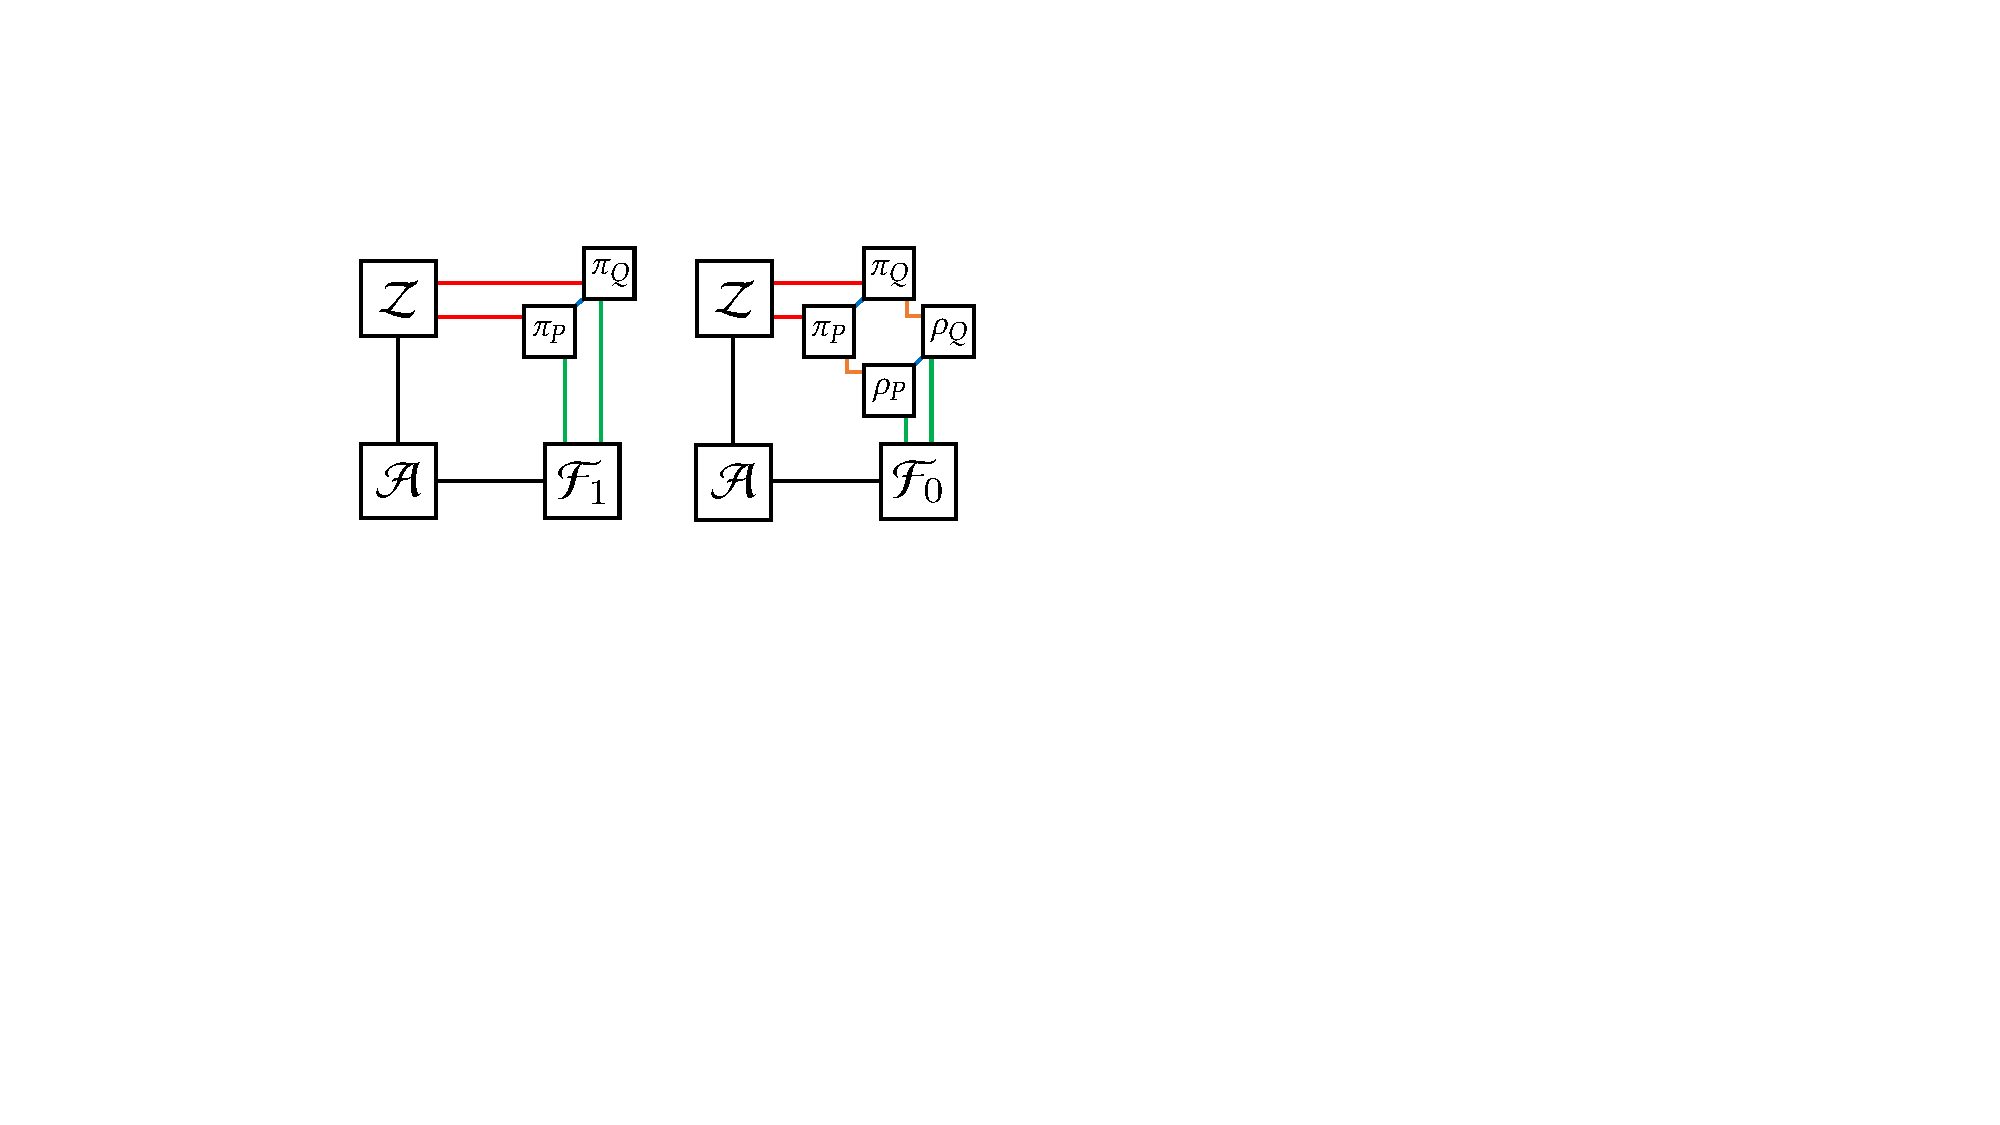
\includegraphics[width=0.85\linewidth]{graphics/protocol-composition}
  \caption{Protocol composition diagram.}
  \label{fig:protocol-composition}
\end{figure}

As a first usage of SaUCy, work through the development of a composition
operator, and give a composition theorem explaining its use.

\todo{Explain more the importance of composition operators}

Essentially, our operator is the notion of UC-realizes. We can now state useful
composition operators, simplifying lemmas, and notation. For brevity, we pack
several notions from UC into a single alternate definition: UC-realizes.

\begin{definition}[UC-realizes]
  Protocol $\pi$ with $\mc{F}_0$ realizes $\mc{F}_1$, written $\mc{F}_0
  \yrightarrow{$\pi$} \mc{F}_1$, if for all environments $\mc{Z}$, if $|-
  \keyword{polyUC}(\mc{Z}, \pi, \mc{F}_0, \mc{A}_{\mathbbm{1}})$, then
  $|- \keyword{polyUC}(\mc{Z}, \pi_{\mathbbm{1}}, \mc{F}_1, \mc{S})$, and the
  following statistical indistinguishability relation holds
  \[ D(\mathsf{execUC}\ \mc{Z}\ \pi\ \mc{F}_0\ \mc{A}_{\mathbbm{1}}) \approx D(\mathsf{execUC}\ \mc{Z}\ \pi_{\mathbbm{1}}\ \mc{F}_1\ \mc{S}).\]
\end{definition}

\todo{The idea is that the environment can arbitrarily and adaptively choose
  inputs to the protocol $\phi$. So when we compose with an arbitrary other
  protocol $\rho$, it is not any worse than what the environment could have
  done. It essentially creates a proof obligation to ensure isolation of the
  protocols.}  While the intended use of universal composition is to replace an
ideal functionality with a protocol that securely realizes it, we define
protocol composition \todo{Let's just call it protocol composition, not
  universal composition. It's not really universal.} more generally in terms of
replacing one subroutine protocol with another. Given a protocol $\phi$, a protocol
$\rho$ that makes calls to $\phi$, \todo{instead of ``makes calls'', specify that the
  \textsf{toF} channel of $\rho$ is connected to the \textsf{fromZ} channel of
  $\phi$. } and a protocol $\pi$ that emulates $\phi$, then $\rho^{\phi -> \pi}$ is identical to
$\rho$ with the following modifications:
\begin{itemize}[leftmargin=*]
  \item When $\rho$ writes to $\phi$, $\rho^{\phi -> \pi}$ writes to $\pi$.
  \item When $\rho^{\phi -> \pi}$ receives a message from $\pi$, proceed as $\rho$ would when
    it receives the same message from $\phi$.
\end{itemize}

\begin{figure}
\lstinputlisting[style=myilc]{listings/compose.ilc}
\caption{Protocol composition operator.}
\label{fig:composition-operator}
\end{figure}

From UC-realizes, we can conclude the original UC formulation for arbitrary
composition:
\begin{theorem}[Composition Theorem]
  If $\mc{F}_0 \yrightarrow{$\pi$} \mc{F}_1$, then for all $\rho$ we
  have that $(\rho^{\pi}, \mc{F}_0)$ emulates $(\rho, \mc{F}_1)$.
\end{theorem}

\subsection{Instantiating UC Commitments}
\label{subsec:example}
We walk through the development of a UC instantiation for commitments.  UC
commitments can be instantiated with standard cryptographic assumptions, for
example the RSA problem.  Also rely on a ``trusted setup'', or common reference
string, essentially public parameters generated ahead of time (modeled as an
ideal functionality FCRS).

Instantiation proofs in UC follow a standard rhythm. We start with a security
definition as an ideal functionality, give the protocol, construct a simulator,
and finally complete the relational analysis on paper.  UC commitments are
reasoned to be secure assuming a common reference string is suitably generated.
To model the cryptography we extend ILC with additional syntax.

The functionality FCom has already been defined.
\todo{Recap the proof obligation}

\paragraph{Extending ILC with cryptographic primitives.}
UC Commitments are realized from cryptographic primitives, such as pseudorandom
trapdoor permutations. This requires us to extend the syntax. The semantics are
written in terms of the cryptographic objects themselves, and we still arrive at
a computational reduction for our security proof.

The new syntactic forms are \textsf{kgen}, \textsf{tdp}, \textsf{inv}, and
\textsf{hc} with the static and dynamic semantics shown in
Figure~\ref{fig:extended-ilc}. The key generation function \textsf{keygen}
generates, on input $1^n$ (security parameter), a random public key $v_{pk}$ and
a trapdoor $v_{td}$. The trapdoor permutation function \textsf{tdp} computes, on
input key $v_k$ and bitstring $v_{in}$, a bitstring $v_{out}$. The hardcore
predicate function \textsf{hc} generates, on input trapdoor permutation
$f_{v_k}$.

\begin{figure*}
  \begin{grammar}
    Expressions
    & $e$
        &$\bnfas$&
        $\eKGen{e} \bnfalt \eTdp{e_1}{e_2} \bnfalt \eHc{e}$
  \end{grammar}
  
  \judgbox{\Delta ; \Gamma |- e : A |> m}{~~Under $\Delta$ and $\Gamma$, expression~$e$ has
  intuitionistic type $A$ and mode $m$.}
  \begin{mathpar}
  \Infer{kgen}
  {\Delta ; \Gamma |- e : [\tyBit]}
  {\Delta; \Gamma |- \eKGen{e}: [\tyBit]}
  %
  \and
  %
  \Infer{eTdp}
  {\Delta_1; \Gamma |- e_1 : [\tyBit]\\
   \Delta_2; \Gamma |- e_2 : [\tyBit]}
  {\Delta_1, \Delta_2; \Gamma |- \eTdp{e_1}{e_2}: [\tyBit]}
  %
  \and
  %
  \Infer{hc}
  {\Delta; \Gamma |- e : \tyArr{[\tyBit]}{}{\tyArr{[\tyBit]}{}{[\tyBit]}}}
  {\Delta; \Gamma |- \eHc{e}: \tyBit}
  \end{mathpar}
  
  \judgbox{\Store_1 ; e_1 ---> \Store_2 ; e_2}{~~Under store $\Store_1$,
    expression~$e_1$ reduces to~$\Store_2 ; e_2$.}
  \begin{mathpar}
  \Infer{kgen}
  {\keyword{\textbf{Gen}}(n) = (v_{pk}, v_{td}) \\ v_{pk}, v_{td} \in \{0,1\}^n}
  { \Store ; \eKGen{n} ---> \Store ; (v_{pk}, v_{td})}
  \and
  \Infer{tdp}
  {\mathbf{f}_{v_k}(v_i) = v_o \\ \mathbf{f} \colon \{0,1\}^n -> \{0,1\}^n -> \{0,1\}^n}
  { \Store ; \eTdp{v_k}{v_i} ---> \Store ; v_o }
  \and
  \Infer{hc}
  {\keyword{\textbf{Hc}}(\mathbf{f}_{v_k}) = v \\ \keyword{\textbf{Hc}} \colon
  (\{0,1\}^n -> \{0,1\}^n) -> \{0, 1\}}
  { \Store ; \eHc{f_{v_k}} ---> \Store ; v}
  \end{mathpar}
%  \begin{mathpar}
%    G_{pk}(r) = (f^{(3n)}_{pk}(r), B(f^{(3n-1)}_{pk}(r)), \ldots, B(f_{pk}(r)), B(r))
%  \end{mathpar}
  \caption{ILC extended with trapdoor permutations.}
  \label{fig:extended-ilc}
\end{figure*}


\begin{algorithm}
\SetAlgorithmName{Protocol}{protocol}{List of Protocols}
\DontPrintSemicolon

\SetKwBlock{Parameters}{\textnormal{\textsf{Public strings}:}}{}
\Parameters{
  $\sigma$: Random string in $\{0,1\}^{4n}$\;
  ${pk}_0, {pk}_1$: Keys for generator $G_{k} \colon \{0,1\}^n \to \{0,1\}^{4n}$
}\smallskip
\SetKwBlock{Commit}{\textnormal{\textsf{Commit}($b$):}}{}
\Commit{
  $r \leftarrow \{0, 1\}^n$\;
  $x \coloneqq G_{{pk}_b}(r)$\;
  if $b=1$ then $x \coloneqq x \oplus \sigma$\;
  Send $(\mathsf{Commit}, x)$ to receiver.\;
  Upon receiving $(\mathsf{Commit}, x)$ from $A$, $B$ outputs $(\mathsf{Receipt})$.
}\smallskip

\SetKwBlock{Decommit}{\textnormal{\textsf{Decommit}($x$):}}{}
\Decommit{
  Send $(b, r)$ to receiver.\;
  Receiver checks $x = G_{{pk}_b}(r)$ for $b = 0$, or $x = G_{{pk}_b}(r) \oplus \sigma$
  for $b = 1$. If verification succeeds, then $B$ outputs $(\mathsf{Open}, b)$.
}
\caption{Universally Composable Commitment}
\label{alg:com}
\end{algorithm}

\begin{figure}
\lstinputlisting[style=myilc]{listings/ucc.ilc}
\caption{Universally composable commitment in ILC.}
\label{fig:ucc}
\end{figure}

\paragraph{Commitment Protocol.}
We defer the protocol to the appendix.

\paragraph{Defining the simulator.}

\paragraph{Relational argument.}

\subsection{Reentrancy in SaUCy}
\label{subsec:reentrancy}

The cryptography community has recently identified several subtleties in defining UC ideal functionalities that relate to ``reentrancy'' and scheduling of concurrent code;
as a consequence, many functionalities in the literature turn out to be ill-defined~\cite{camenisch2016universal}.
This subtle definitional issue, although important for the well-foundedness of security claims,
is not ``cryptographic'' in nature, and is better addressed from the PL viewpoint.
To illustrate, consider the following fragment of (untyped) ILC syntax, which allows an adversary to control the delivery schedule of messages from $P$ to $Q$ (an asynchronous channel):
\lstinputlisting[style=myilc]{listings/reentrant.ilc}
After receiving input from party $P$, it
notifies the adversary, then forks a background thread to wait for \textsf{OK} before
delivering the message.
This introduces a race condition: suppose input message $m_1$ is sent by $P$, but then the adversary $\mathcal A$, before sending \textsf{OK}, instead returns control to $\mathcal Z$, which passes $P$ a second input $m_2$. Now there are two queued messages; which one gets delivered first when the adversary sends \textsf{OK}?

To resolve this paradox, notice that fragment is untypeable in ILC.
The race condition occurs because of duplication of the read channel \textsf{frA}.
Since \textsf{frA} is linear in the function body, the function would not be typeable as intuitionistic as required by the \textsf{loop} construct.
Camenisch et al.~\cite{camenisch2016universal} identified several strategies for resolving this problem in UC, which in turn are expressible ILC. One approach is to make the process explicitly sequential, such that the arrival of a second message before the first is delivered causes execution to get stuck:
\lstinputlisting[style=myilc]{listings/reentrant-seq.ilc}
An alternative is to discard such messages arriving out of order, returning them to sender; this can be expressed in ILC using the external choice operator:
operator,
\lstinputlisting[style=myilc]{listings/reentrant-ignore.ilc}
